% !TEX outputDirectory = _build
\documentclass[10pt,a4paper]{article}
\usepackage[T1]{fontenc}
\usepackage[utf8]{inputenc}
% \usepackage[a4paper,margin=1.8cm]{geometry}
\usepackage{multicol}
\usepackage{xcolor}
\usepackage{array}
\usepackage{titlesec}
\usepackage[hidelinks]{hyperref}
\usepackage{graphicx}
\usepackage{eso-pic}
\usepackage{tikz}
\usetikzlibrary{calc}
\usepackage[export]{adjustbox}
\usepackage{xurl}
\usepackage{multirow}
\usepackage{wrapfig}

\definecolor{conf}{HTML}{023E8A}
\titleformat{\section}{\color{conf}\Large\bfseries}{}{0em}{}
\pagestyle{empty}
\setlength{\parindent}{0pt}

\usepackage{enumitem}
\usepackage{longtable}
\usepackage[table]{xcolor}
\usepackage{tabularx}
\usepackage{hyperref}
% Define custom colors
\definecolor{lightgraybg}{gray}{0.94}
\definecolor{linkblue}{RGB}{0, 102, 204}
% Set up hyperref styling
\hypersetup{
    colorlinks=true,
    urlcolor=linkblue
}


\usepackage[a4paper, margin=1.8cm, top=1cm, headheight=1cm, headsep=20pt, includehead]{geometry}
\usepackage{graphicx}
\usepackage{fancyhdr}

% --- Define the default header/footer style ---
% \pagestyle{fancy}
% \fancyhf{} % Clear existing defaults
% % \rhead = top right, \lhead = top left, \chead = center
% \rhead{
\includegraphics[height=10pt]{images/iwbis_logo.png}} % image in header
% \lhead{IWBIS 2026 | PROGRAM BOOK}

% Header and footer style
\pagestyle{fancy}
\fancyhf{} % Clear existing defaults

% Header
\lhead{IWBIS 2026 | PROGRAM BOOK}
\rhead{
\includegraphics[height=10pt]{images/iwbis_logo.png}}

% Footer
\cfoot{\textcolor{conf}{\small\thepage}}

% Optional: remove the default horizontal line below the header
\renewcommand{\headrulewidth}{0pt}

% Optional: add a subtle line above the footer
\renewcommand{\footrulewidth}{0.4pt}

\begin{document}

% ======== COVER
\thispagestyle{empty}
\AddToShipoutPictureBG*{%
  \includegraphics[width=\paperwidth,height=\paperheight]{assets/background.pdf}%
}

\begin{tikzpicture}[remember picture, overlay]

  \node[anchor=north, inner sep=0pt]
    at ([yshift=-3cm]current page.north)
    {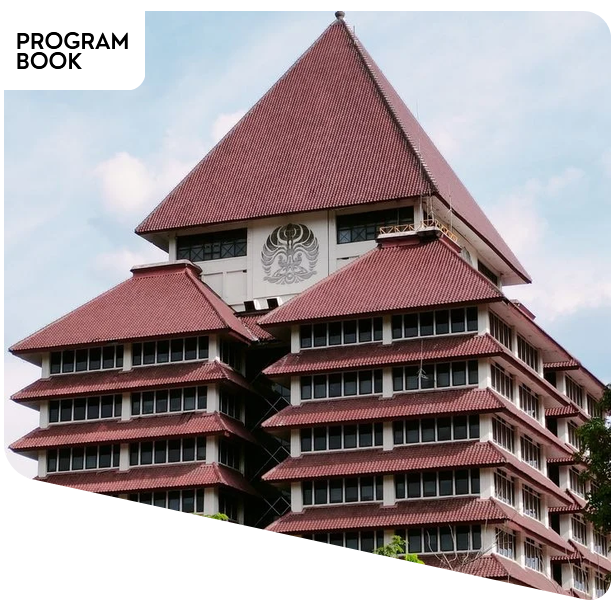
\includegraphics[width=15cm]{images/cover_image.png}};

  \node[anchor=north, inner sep=0pt]
    at ([yshift=-18.5cm]current page.north)
    {
\includegraphics[width=10cm]{images/iwbis_logo.png}};

  \node[anchor=north, text width=150mm, align=justify]
    at ([yshift=-20cm]current page.north)
    {\Large The $15^{th}$  International Workshop on Big Data and Information Security (IWBIS) provides an international forum that brings together those who are actively involved in the field of Big Data and Information Security.};

  \node[anchor=north, text width=150mm, align=center]
    at ([xshift=-6cm, yshift=-23.25cm]current page.north)
    {\large Host};

  \node[anchor=north, text width=150mm, align=center]
    at ([xshift=-1.5cm, yshift=-23.25cm]current page.north)
    {\large Financial Sponsor};

  \node[anchor=north, text width=150mm, align=center]
    at ([xshift=4cm, yshift=-23.25cm]current page.north)
    {\large Technical Sponsor};
  
  \node[anchor=north, inner sep=0pt]
    at ([yshift=-24cm]current page.north)
    {
\includegraphics[width=15cm]{images/sponsors.png}};


  \draw[gray, line width=0.5pt] (5, -20) -- (5, -24);  
  \draw[gray, line width=0.5pt] (9.5, -20) -- (9.5, -24);  
    
\end{tikzpicture}
% Conf info ====================================================
\newpage
\vspace*{1cm}
\hspace{1cm}{\LARGE \textbf{CONFERENCE INFORMATION}}

\noindent
% Set cell padding
\renewcommand{\arraystretch}{1.3}
\setlength{\tabcolsep}{14pt}

\begin{center}
\begin{tabularx}{0.85\textwidth}{@{}>{\raggedright\arraybackslash}p{3.4cm} >{\raggedright\arraybackslash}X@{}}
  
  \rowcolor{lightgraybg} & \\[-6pt] % top padding
  
  % Apply light gray background to the entire table
  \rowcolor{lightgraybg}
  Dates & October 16\textsuperscript{th} (Friday) -- October 18\textsuperscript{th} (Sunday) 2026 \\[4pt]
  
  \rowcolor{lightgraybg}
  Organizer & \textbf{Faculty of Computer Science, Universitas Indonesia}, Indonesia \\
  \rowcolor{lightgraybg}
  & \textbf{Universitas Pertahanan}, Indonesia \\[4pt]
  
  \rowcolor{lightgraybg}
  Venue & Auditorium Indro Suwandi \\[10pt]
  
  \rowcolor{lightgraybg}
  Official Language & English \\[4pt]
  
  \rowcolor{lightgraybg}
  Secretariat & Faculty of Computer Science, Universitas Indonesia \\
  \rowcolor{lightgraybg}
  & Kampus UI Depok \\
  \rowcolor{lightgraybg}
  & Depok, 16424 \\
  \rowcolor{lightgraybg}
  & Indonesia \\
  \rowcolor{lightgraybg}
  & T: +62 21786 3419 ext. 3225 \\
  \rowcolor{lightgraybg}
  & F: +62 21 786 3415 \\
  \rowcolor{lightgraybg}
  & E: iwbis@cs.ui.ac.id \\
  \rowcolor{lightgraybg}
  & W: \url{https://www.cs.ui.ac.id} \\[10pt]
  
  \rowcolor{lightgraybg}
  Conference Website & \url{https://iwbis.cs.ui.ac.id} \\

  
  \rowcolor{lightgraybg} & \\[-6pt] % Bottom padding row
\end{tabularx}
\end{center}

% Agenda =======================================================
\newpage
\begin{center}
  {\color{conf}\fontsize{36}{40}\selectfont\bfseries IWBIS 2026}\\[0.2em]
  {\Large International Workshop on Big Data and Information Security}\\[0.2em]
  {\large October 16--18, 2026 \;•\; Depok, Indonesia \;•\; https://iwbis.cs.ui.ac.id/}
\end{center}

\vspace{0.5em}
\color{conf}\rule{\linewidth}{1pt}\color{black}

\begin{multicols}{2}

\section*{Day 1 -- Friday, 16 Oct}
\textbf{15:30 -- 18:30}~~Early Welcoming Dinner for Speakers\\
\hspace*{2em}\textcolor{gray}{Margo Hotel (Tentative)}\\
\hspace*{2em}\textcolor{gray}{Kemungkinan 40 orang}

\section*{Day 2 -- Saturday, 17 Oct}
\textbf{07:00 -- 08:00}~~Registration Desk Open\\
\hspace*{2em}\textcolor{gray}{Auditorium Indro Suwandi}\\
\textbf{08:00 -- 08:15}~~Opening Ceremony (Dean)\\
\hspace*{2em}\textcolor{gray}{Auditorium Indro Suwandi}\\
\textbf{08:15 -- 09:15}~~Keynote 1: Prof. Mahardika (ICACSIS)\\
\hspace*{2em}\textcolor{gray}{Auditorium Indro Suwandi}\\
\textbf{09:15 -- 10:15}~~Keynote 2: Prof. Raj Kumar Buyya\\
\hspace*{2em}\textcolor{gray}{Auditorium Indro Suwandi}\\
\textbf{10:15 -- 10:30}~~Coffee Break\\
\hspace*{2em}\textcolor{gray}{Selasar Auditorium}\\
\textbf{10:30 -- 11:30}~~Keynote 3: Pak Fauzan\\
\hspace*{2em}\textcolor{gray}{Auditorium Indro Suwandi}\\
\textbf{11:30 -- 12:30}~~Keynote 4: Warek 3 \emph{(Parallel)}\\
\hspace*{2em}\textcolor{gray}{Kelas Lt. 2 Zona 3}\\
\textbf{12:30 -- 13:10}~~Break + Lunch\\
\hspace*{2em}\textcolor{gray}{Selasar Auditorium, Lunch Prasmanan (pisah antara VIP dan peserta)}\\
\textbf{13:10 -- 13:40}~~Keynote 5: Rektor UI\\
\hspace*{2em}\textcolor{gray}{Auditorium Indro Suwandi}\\
\textbf{13:40 -- 14:10}~~Keynote 6: Prof. Arif Satria\\
% \hspace*{2em}\emph{(minta bantuan sekpim; just in case gak bisa, pake delegasi/utusan/perwakilan dari beliau atau rekaman; disampaikan di undangan)}\\
\hspace*{2em}\textcolor{gray}{Auditorium Indro Suwandi}\\
\textbf{14:10 -- 14:25}~~Coffee Break\\
\hspace*{2em}\textcolor{gray}{Selasar Auditorium}\\
\textbf{14:25 -- 15:25}~~Keynote 7: Prof. Simon See\\
\hspace*{2em}\textcolor{gray}{Auditorium Indro Suwandi}\\
\textbf{15:25 -- 16:05}~~Break\\
\hspace*{2em}\textcolor{gray}{Selasar Auditorium}\\
\textbf{16:05 -- 16:50}~~Invited Speaker 1 ICACSIS (Henry) + Invited Speaker 1 IWBIS (Kamrul Hasan) \emph{(Parallel)}\\
\hspace*{2em} \textcolor{gray}{Ruang Sidang}\\
\textbf{16:50 -- 17:35}~~Keynote 8: Prof. Andrea Acquaviva -- online\\
\hspace*{2em}\textcolor{gray}{Auditorium Indro Suwandi}\\
\textbf{19:00 -- 21:00}~~Gala Dinner \& Best Paper Award\\
\hspace*{2em}\textcolor{gray}{Selasar Auditorium, Seluruh Peserta, Award Best Paper}

\section*{Day 3 -- Sunday, 18 Oct}
\textbf{08:00 -- 09:45}~~Registration \& Opening \emph{(Parallel)}\\
\hspace*{2em}\textcolor{gray}{Ruang Sidang Lt. 4}\\
\textbf{09:45 -- 10:00}~~Coffee Break\\
\hspace*{2em}\textcolor{gray}{Selasar Auditorium}\\
\textbf{10:00 -- 11:45}~~Parallel Sessions \emph{(Parallel)}\\
\hspace*{2em}\textcolor{gray}{3 classroom}\\
\textbf{11:45 -- 12:45}~~Break\\
\textbf{12:45 -- 13:30}~~Keynote 1: Prof. Subhas \emph{(Parallel)}\\
\hspace*{2em}\textcolor{gray}{Auditorium Indro Suwandi}\\
\textbf{14:15 -- 15:00}~~Keynote 1: Prof. T.M Indra Mahlia \emph{(Parallel)}\\
\hspace*{2em}\textcolor{gray}{Auditorium Indro Suwandi}\\
\textbf{15:00 -- 16:00}~~Coffee Break\\
\hspace*{2em}\textcolor{gray}{Selasar Auditorium}\\
\textbf{16:00 -- 16:45}~~Invited Speaker 1: Grafika \emph{(Online)}\\
\hspace*{2em}\textcolor{gray}{Auditorium Indro Suwandi}\\
\textbf{16:45 -- 17:30}~~Keynote 4: Prof. Xiao \emph{(Online)}\\
\hspace*{2em}\textcolor{gray}{Auditorium Indro Suwandi}\\
\textbf{17:30 -- 18:00}~~Closing \& Award (Best Presenter)

\section*{Venue}
\textbf{Auditorium Indro Suwandi, Gedung Baru FASILKOM}\\
\\
Universitas indonesia, New Building, Fasilkom  UI Jl. Prof. DR. Sudjono D. Pusponegoro 2nd Floor, Pondok Cina, Beji, Depok City, West Java 16424

% \section*{Organizers}
% \textbf{Honorary Chairs:} Heri Hermansyah, Wisnu Jatmiko\\
% \textbf{General Chair:} Harry Budi Santoso\\
% \textbf{Program Chair:} Baginda Anggun Nan Cenka\\
% \textbf{Publicity Chair:} Jessica Naraiswari Arwidarasti\\
% \textbf{Proceeding Chair:} Aprinaldi\\
% \textbf{Treasurer:} Anggitha Woelandhary, Edina Ayuningtyas\\
% \textbf{Local Organizing Chair:} Nandhita Zefania Maharani\\
% \textbf{Program Committee:} Alfan Farizki Wicaksono, Achmad Nizar Hidayanto, Aniati Murni Arymurthy, Ari Saptawijaya, Amril Syalim, Ari Wibisono, Bayu Anggorojati, Betty Purwandari, Dina Chahyati, Erdefi Rakun, Evi Yulianti, Fatimah Azzahro, Fariz Darari, Ika Alfina, Indra Budi, Imairi Eitiveni, Kurniawati Azizah, Laksmita Rahadianti, Lim Yohanes Stefanus, Martin Schrepp, Muhammad Anwar Ma'sum, Muhammad Febrian Rachmadi, Muhammad Okky Ibrohim, Nabila Clydea Harahap, Oenardi Lawanto, Panca Hadi Putra, Rahmad Mahendra, Satrio Pradono Suryodiningrat, Setiadi Yazid, Toto Haryanto, Tsukasa Hirashima, Wahyu Catur Wibowo, Widijanto Satyo Nugroho

\end{multicols}

% ==================== 
% Organizers
% ====================
\clearpage
\section*{\textbf{Organizers \& Committees}}
\color{conf}\rule{\linewidth}{1pt}\color{black}
\vspace{0.5em}
\begin{multicols}{2}
\raggedcolumns

\begin{minipage}{\linewidth}
\textbf{\color{conf}Honorary Chairs}\\
Heri Hermansyah, \textcolor{gray}{Universitas Indonesia, ID}\\
Wisnu Jatmiko, \textcolor{gray}{Universitas Indonesia, ID}
\end{minipage}
\vspace{0.8em}

\begin{minipage}{\linewidth}
\textbf{\color{conf}General Chair}\\
Indra Budi, \textcolor{gray}{Universitas Indonesia, ID}\\
\end{minipage}
\vspace{0.8em}

\begin{minipage}{\linewidth}
\textbf{\color{conf}Program Chair}\\
Vektor Dewanto, \textcolor{gray}{Universitas Indonesia, ID}\\
Ibad Rahadian Saladdin, \textcolor{gray}{Universitas Indonesia, ID}
\end{minipage}
\vspace{0.8em}

\begin{minipage}{\linewidth}
\textbf{\color{conf}Publicity Chair}\\
Jessica Naraiswari Arwidarasti, \textcolor{gray}{Universitas Indonesia, ID}\\
\end{minipage}
\vspace{0.8em}

\begin{minipage}{\linewidth}
\textbf{\color{conf}Proceeding Chair}\\
Lintang Matahari Hasani, \textcolor{gray}{Universitas Indonesia, ID}\\
\end{minipage}
\vspace{0.8em}

\begin{minipage}{\linewidth}
\textbf{\color{conf}Treasurers}\\
Edina Ayuningtyas, \textcolor{gray}{Universitas Indonesia, ID}\\
Nurul Fazriah, \textcolor{gray}{Universitas Indonesia, ID}\\
\end{minipage}
\vspace{0.8em}

\begin{minipage}{\linewidth}
\textbf{\color{conf}Local Organizing Chair}\\
Shabrina Salsabila Kurniawan, \textcolor{gray}{Universitas Indonesia, ID}\\
\end{minipage}
\vspace{0.8em}

\begin{minipage}{\linewidth}
\textbf{\color{conf}Program Committees}\\
Achmad Nizar Hidayanto, \textcolor{gray}{Universitas Indonesia, ID}\\
Alfan Farizki Wicaksono, \textcolor{gray}{Universitas Indonesia, ID}\\
Amril Syalim, \textcolor{gray}{Universitas Indonesia, ID}\\
Ananto Tri Sasongko, \textcolor{gray}{Universitas Pelita Bangsa, ID}\\
Aniruddha Singh Gautam, \textcolor{gray}{Microsoft, US}\\
Anita Hidayati, \textcolor{gray}{Politeknik Negeri Jakarta, ID}\\
Arfive Gandhi, \textcolor{gray}{Universitas Telkom, ID}\\
Ari Saptawijaya, \textcolor{gray}{Universitas Indonesia, ID}\\
Ari Wibisono, \textcolor{gray}{Universitas Indonesia, ID}\\
Ario Yudo Husodo, \textcolor{gray}{Universitas Mataram, ID}\\
Ati Suci Dian Martha, \textcolor{gray}{Telkom University, ID}\\
Avinanta Tarigan, \textcolor{gray}{Universitas Gunadarma, ID}\\
Berliyanto, \textcolor{gray}{Institut Teknologi Budi Utomo, ID}\\
Betty Purwandari, \textcolor{gray}{Universitas Indonesia, ID}\\
Bety Hayat Susanti, \textcolor{gray}{Politeknik Siber dan Sandi Negara, ID}\\
Bayu Anggorojati, \textcolor{gray}{Monash University, ID}\\
Dina Chahyati, \textcolor{gray}{Universitas Indonesia, ID}\\
Erdefi Rakun, \textcolor{gray}{Universitas Indonesia, ID}\\
Esa Prakarsa, \textcolor{gray}{National Research and Innovation Agency, ID}\\
Evi Yulianti, \textcolor{gray}{Universitas Indonesia, ID}\\
Fatimah Azzahro, \textcolor{gray}{Universitas Indonesia, ID}\\
Fariz Darari, \textcolor{gray}{Universitas Indonesia, ID}\\
Ika Alfina, \textcolor{gray}{Universitas Indonesia, ID}\\
Imairi Eitiveni, \textcolor{gray}{Universitas Indonesia, ID}\\
Kurniawati Azizah, \textcolor{gray}{Universitas Indonesia, ID}\\
Laksmita Rahadianti, \textcolor{gray}{Universitas Indonesia, ID}\\
Lim Yohanes Stefanus, \textcolor{gray}{Universitas Indonesia, ID}\\
Muhammad Anwar Ma'sum, \textcolor{gray}{Universitas Indonesia, ID}\\
Muhammad Febrian Rachmadi, \textcolor{gray}{Universitas Indonesia, ID}\\
Muhammad Okky Ibrohim, \textcolor{gray}{Universitas Indonesia, ID}\\
Nabila Clydea Harahap, \textcolor{gray}{Universitas Indonesia, ID}\\
Rahmad Mahendra, \textcolor{gray}{Universitas Indonesia, ID}\\
Santosh Appachu Devanira Poovaiah, \textcolor{gray}{NVIDIA, US}\\
Sarath Kumar Kallayil Sreedharan, \textcolor{gray}{AWS, US}\\
Setiadi Yazid, \textcolor{gray}{Universitas Indonesia, ID}\\
Toto Haryanto, \textcolor{gray}{Institut Pertanian Bogor, ID}\\
Vatsal Gupta, \textcolor{gray}{Apple Inc., US}\\
Wahyu Catur Wibowo, \textcolor{gray}{Universitas Indonesia, ID}\\
Widijanto Satyo Nugroho, \textcolor{gray}{Universitas Indonesia, ID}\\
\end{minipage}
\vspace{0.8em}
\end{multicols}

% ==================== 
% STUDENT VOLUNTEERS 
% ====================
\clearpage
\section*{\textbf{Student Volunteers}}
\color{conf}\rule{\linewidth}{1pt}\color{black}
\vspace{0.5em}
\begin{multicols}{2}
\raggedcolumns

% Team 1
\begin{minipage}{\linewidth}
\textbf{\color{conf}Volunteer Coordinator} \textcolor{gray}{\emph{All Area}}\\
Riri Safitri \textcolor{gray}{(S3 - 2025)}\\ 
Suryatiningsih \textcolor{gray}{(S3 - 2025)}\\ 
Yogiek Indra Kurniawan \textcolor{gray}{(S3 - 2024)}\\
Muhammad Naufal Al Ghifari \textcolor{gray}{(S2 - 2025)}\\
\end{minipage}
\vspace{0.8em}

% Team 2
\begin{minipage}{\linewidth}
\textbf{\color{conf}Registration \& Welcome Desk}\\
\textcolor{gray}{\emph{Registration Area}}\\
\small \underline{Lead: Ayreine Nisya' D} \textcolor{gray}{(S2 - 2025)}\\
\begin{itemize}\setlength{\itemsep}{0pt}
  \item Ahmad Rizki Daffaa \textcolor{gray}{(S1 - 2025)}
  \item Fadil Surya Pramana \textcolor{gray}{(S1 - 2026)}
  \item Vanessa Josephin Gwi \textcolor{gray}{(S1 - 2026)}
\end{itemize}
\end{minipage}
\vspace{0.8em}

% Team 3
\begin{minipage}{\linewidth}
\textbf{\color{conf}Information Desk \& Participant Service}\\\textcolor{gray}{\emph{Lobby / Help Desk}}\\
\small \underline{Lead: Syaikha Amirah Zikrina} \textcolor{gray}{(S2 - 2025)}\\
\begin{itemize}\setlength{\itemsep}{0pt}
  \item Hilda Nida Alistiqlal \textcolor{gray}{(S2 - 2025)}
  \item Farel Boston Corinthians Nadeak \textcolor{gray}{(S1 - 2025)}
\end{itemize}
\end{minipage}
\vspace{0.8em}

% Team 4
\begin{minipage}{\linewidth}
\textbf{\color{conf}VIP \& Speaker Liaison}\\
\textcolor{gray}{\emph{VIP / Speaker Area}}\\
\small \underline{Lead: Suryatiningsih} \textcolor{gray}{(S3 - 2025)}\\
\begin{itemize}\setlength{\itemsep}{0pt}
  \item Muhammad Kaddafi Suyatno \textcolor{gray}{(S2 - 2025)}
  \item Muhammad Naufal Al Ghifari \textcolor{gray}{(S2 - 2025)}
  \item Hilda Nida Alistiqlal \textcolor{gray}{(S2 - 2025)}
  \item Vanessa Josephin Gwi \textcolor{gray}{(S1 - 2026)}
\end{itemize}
\end{minipage}
\vspace{0.8em}

% Team 5
\begin{minipage}{\linewidth}
\textbf{\color{conf}Session Chair}\\
\textcolor{gray}{\emph{Parallel Session Room}}\\
\small \underline{Lead: Nashuha Insani} \textcolor{gray}{(S2 - 2025)}\\
\begin{itemize}\setlength{\itemsep}{0pt}
  \item Agsanshina Raka Syakti \textcolor{gray}{(S2 - 2024)}
  \item Tasya Mulia Salsabila \textcolor{gray}{(S2 - 2025)}
  \item Nabila Hermawati \textcolor{gray}{(S2 - 2026)}
\end{itemize}
\end{minipage}
\vspace{0.8em}

% Team 6
\begin{minipage}{\linewidth}
\textbf{\color{conf}Parallel Session Room Assistant}\\
\textcolor{gray}{\emph{Parallel Session Room}}\\
\small \underline{Lead: Muhammad Kaddafi Suyatno} \textcolor{gray}{(S2 - 2025)}\\
\begin{itemize}\setlength{\itemsep}{0pt}
  \item Mikhael Tobias Ezra Simanjuntak \textcolor{gray}{(S1 - 2026)}
  \item Rindivia Derilla Zihan \textcolor{gray}{(S1 - 2026)}
\end{itemize}
\end{minipage}
\vspace{0.8em}

% Team 7
\begin{minipage}{\linewidth}
\textbf{\color{conf}Technical Support}\\
\textcolor{gray}{\emph{All Session Room}}\\
\small \underline{Lead: Vincentius Filbert Amadeo} \textcolor{gray}{(S1 - 2024)}\\
\begin{itemize}\setlength{\itemsep}{0pt}
  \item Fahrezy Khairu Ghassani \textcolor{gray}{(S1 - 2026)}
  \item Almas Mustaqim
\end{itemize}
\end{minipage}
\vspace{0.8em}

% Team 8
\begin{minipage}{\linewidth}
\textbf{\color{conf}Time Keeper}\\
\textcolor{gray}{\emph{Session Room}}\\
\small \underline{Lead: Harman Hakim} \textcolor{gray}{(S1 - 2023)}\\
\begin{itemize}\setlength{\itemsep}{0pt}
  \item Daffa Mohamad Fathoni \textcolor{gray}{(S1 - 2022)}
\end{itemize}
\end{minipage}
\vspace{0.8em}

% Team 9
\begin{minipage}{\linewidth}
\textbf{\color{conf}Auditorium Main Hall}\\
\textcolor{gray}{\emph{Main Auditorium}}\\
\small \underline{Lead: Riri Safitri} \textcolor{gray}{(S3 - 2025)}\\
\begin{itemize}\setlength{\itemsep}{0pt}
  \item Yogiek Indra Kurniawan \textcolor{gray}{(S3 - 2024)}
  \item Muhammad Naufal Al Ghifari \textcolor{gray}{(S2 - 2025)}
\end{itemize}
\end{minipage}
\vspace{0.8em}

% Team 10
\begin{minipage}{\linewidth}
\textbf{\color{conf}Documentation \& Media}\\
\textcolor{gray}{\emph{All Venue}}\\
\small \underline{Lead: Nadya Aulia Putri} \textcolor{gray}{(S2 - 2024)}\\
\begin{itemize}\setlength{\itemsep}{0pt}
  \item Alif Shidqi Putra Amir \textcolor{gray}{(S1 - 2025)}
  \item Glenn Josia Devano \textcolor{gray}{(S1 - 2025)}
  \item Batrisya Dayana \textcolor{gray}{(S1 - 2026)}
\end{itemize}
\end{minipage}
\vspace{0.8em}

% Team 11
\begin{minipage}{\linewidth}
\textbf{\color{conf}Hospitality \& Catering}\\
\textcolor{gray}{\emph{Lunch / Coffee Break / Gala Dinner}}\\
\small \underline{Lead: Hilda Nida Alistiqlal} \textcolor{gray}{(S2 - 2025)}\\
\begin{itemize}\setlength{\itemsep}{0pt}
  \item Vanessa Josephin Gwi \textcolor{gray}{(S1 - 2026)}
  \item Farel Boston Corinthians Nadeak \textcolor{gray}{(S1 - 2025)}
  \item Muhammad Kaddafi Suyatno \textcolor{gray}{(S2 - 2025)}
  \item Rindivia Derilla Zihan \textcolor{gray}{(S1 - 2026)}
\end{itemize}
\end{minipage}
\vspace{0.8em}

\end{multicols}

% ==================== 
% Speakers
% ====================
\clearpage
\section*{\textbf{Speakers}}
\color{conf}\rule{\linewidth}{1pt}\color{black}
\vspace{0.5em}
\noindent

% % --- LEFT COLUMN ---
\large{\textbf{KEYNOTE SPEAKER}}\\
\begin{minipage}[t]{0.25\textwidth}
    \vspace{0pt}% <-- aligns top of minipage with top of the other one
    
    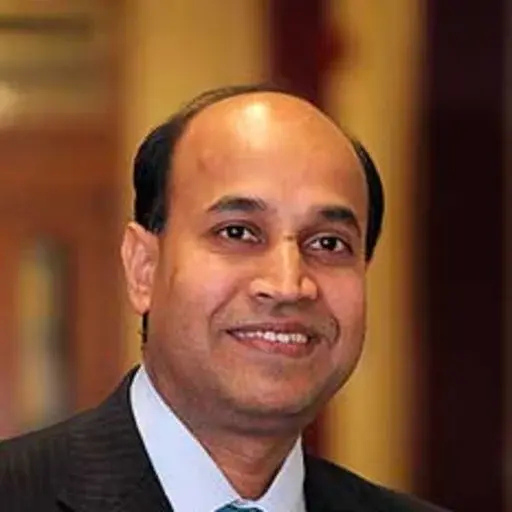
\includegraphics[width=\linewidth]{images/portraits/subhas_mukhopadhyay.png} \\[0.5em]
    \begin{center}
        {\normalsize \textbf{PROF. DR. SUBHAS MUKHOPADHYAY, FIEE, FIETE}} \\[1em]
        {\normalsize Professor of Mechanical/Electronics Engineering} \\[1em]
        {\normalsize \textbf{School of Engineering, Macquarie University, NSW 2109 Australia}}   
    \end{center}
\end{minipage}%
\hfill
% --- RIGHT COLUMN ---
\begin{minipage}[t]{0.72\textwidth}
    \vspace{0pt}% <-- same trick on the right column
    
    Subhas holds a B.E.E. (gold medallist), M.E.E., Ph.D. (India) and Doctor of Engineering (Japan). He has over 35+ years of teaching, industrial and research experience. Currently he is working as a Professor of Mechanical/Electronics Engineering, Macquarie University, Australia and is the Discipline Leader of the Mechatronics Engineering Degree Programme. His fields of interest include Smart Sensors and sensing technology, instrumentation techniques, wireless sensors and network (WSN), Internet of Things (IoT), robotics and Mechatronics, and Drones etc. He has supervised over 60 postgraduate students and over 200 Honours students. He has examined over 80 postgraduate theses.
    
    \vspace{1em} % Space between paragraphs
    
    He has been co-inventor of 14 patents and published over 500 papers in different international journals and conference proceedings, written ten books and sixty two book chapters and edited twenty conference proceedings. He has also edited fifty books and forty five journal special issues. He has organized over 25 international conferences as either General Chairs/co-chairs or Technical Programme Chair. He has delivered 470 presentations including keynote, invited, tutorial and special lectures. As per Google Scholar, his total citation is 30965 and h-index is 89.
    
    \vspace{1em}
    
    He is a Fellow of IEEE (USA), a Fellow of IET (UK), a Fellow of IETE (India). He was a Topical Editor of IEEE Sensors Journal from 2013 to 2025 and an Associate Editor for IEEE Transactions on Instrumentation and Measurements from 2007 to 2025. He is an associate editor of IEEE Transactions on Reviews in Biomedical Engineering (RBME). He is the EiC of the International Journal on Smart Sensing and Intelligent Systems. He was a Distinguished Lecturer of the IEEE Sensors Council from 2017 to 2022. He chairs the IEEE Instrumentation and Measurement Society NSW chapter.

    \vspace{1em}

    For more details, please see:
    \begin{itemize}
        \item \url{https://scholar.google.com.au/citations?user=8p-BvWIAAAAJ\&hl=en} 
        \item \url{https://orcid.org/0000-0002-8600-5907} 
        \item \url{http://web.science.mq.edu.au/directory/listing/person.htm?id=smukhopa}
    \end{itemize}
\end{minipage}

% ======================================================================================
\newpage
% % --- LEFT COLUMN ---
\large{\textbf{KEYNOTE SPEAKER}}\\
\begin{minipage}[t]{0.25\textwidth}
    \vspace{0pt}%
    
    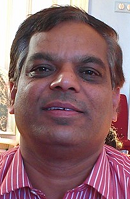
\includegraphics[width=\linewidth]{images/portraits/rajkumar_buyya.png} \\[0.5em]
    \begin{center}
        {\textbf{PROF. RAJKUMAR BUYYA}} \\[1em]
        {\normalsize Fellow of ACM, IEEE, and Academia Europaea Director, Cloud Computing and Distributed Systems (CLOUDS) Lab CEO} \\[1em]
        {\normalsize \textbf{The University of Melbourne, Australia\\ Manjrasoft Pvt Ltd, Melbourne, Australia}}   
    \end{center}
\end{minipage}%
\hfill
% --- RIGHT COLUMN ---
\begin{minipage}[t]{0.72\textwidth}
    \vspace{0pt}% 
    
    Dr. Rajkumar Buyya is a Redmond Barry Distinguished Professor and Director of the Quantum Cloud Computing and Distributed Systems (qCLOUDS) Laboratory at the University of Melbourne, Australia. He is also serving as the founding CEO of Manjrasoft, a spin-off company of the University, commercializing its innovations in Cloud Computing. He has authored over 850 publications and seven textbooks including “Mastering Cloud Computing” published by McGraw Hill, China Machine Press, and Morgan Kaufmann for Indian, Chinese and international markets respectively. Dr. Buyya is one of the highly cited authors in computer science and software engineering worldwide (h-index=181, g-index=394, i10-index=891, and 172,600+ citations). A bibliometric study by Stanford University and Elsevier since 2019, Dr. Buyya is recognized as the Highest-Cited author in the Distributed Computing field worldwide. He graduated 66+ PhD students who are working in world-leading research universities and high-tech companies such as Microsoft, Google, and IBM. He has been recognised as an ACM Fellow, IEEE Fellow, Fellow of the Academy of Europe, a “Web of Science Highly Cited Researcher” for seven times since 2016, the “Best of the World” twice for research fields (in Computing Systems in 2019/2024 and Software Systems in 2021/2022/2023) as well as “Lifetime Achiever” and “Superstar of Research” in “Engineering and Computer Science” discipline twice (2019 and 2021) by the Australian Research Review.

    \vspace{1em}

    Software technologies for Grid, Cloud, Fog, Quantum computing developed under Dr.Buyya’s leadership have gained rapid acceptance and are in use at several academic institutions and commercial enterprises in 60+ countries around the world. Manjrasoft’s Aneka Cloud technology developed under his leadership has received “Frost New Product Innovation Award”. He served as founding Editor-in-Chief of the IEEE Transactions on Cloud Computing. He is currently serving as Editor-in-Chief of Software: Practice and Experience, a long-standing journal in the field established in 1970. He has presented over 750 invited talks (keynotes, tutorials, and seminars) on his vision on IT Futures, Advanced Computing technologies, and Spiritual Science at international conferences and institutions in Asia, Australia, Europe, North America, and South America. 
    
    \vspace{1em}
    
    For further information on Dr. Buyya, please visit his cyberhome: \url{www.buyya.com }
\end{minipage}
% ======================================================================================
\newpage
% --- LEFT COLUMN ---
\large{\textbf{KEYNOTE SPEAKER}}\\
\begin{minipage}[t]{0.25\textwidth}
    \vspace{0pt}%
    
    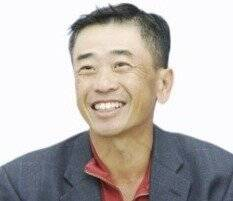
\includegraphics[width=\linewidth]{images/portraits/simon_see.png} \\[0.5em]
    \begin{center}
        {\textbf{PROF. SIMON SEE}} \\[1em]
        {\normalsize \textbf{Director\\[0.5em]NVIDIA AI Technology Center USA}}   
    \end{center}
\end{minipage}%
\hfill
% --- RIGHT COLUMN ---
\begin{minipage}[t]{0.72\textwidth}
    \vspace{0pt}% 
    Professor Simon See is currently the Solution Architecture and Engineering Senior Director, Chief Solution Architect \& Global Head for Nvidia AI Technology Center, NVIDIA Corporation. He is also a Professor at Shanghai Jiao Tong University, Professor in Beijing University of Posts and Telecommunications (BUPT), and Professor in Universitas Indonesia (UI). He is being conferred as a Distinguished Fudan Scholar in September 2018 by Fudan University, Shanghai, China. Previously Professor See is also the Chief Scientific Computing Advisor for BGI (China) and has a position in Nanyang Technological University (Singapore) and King-Mong Kung University of Technology (Thailand). Professor See is currently involved in a number of International computational, mathematical science projects and national AI initiatives. Recently Dr Simon has been appointed as the Executive Director of the ASEAN Applied Research Centre (AARC). His research interests are in the area of High-Performance Computing, Big Data, Artificial Intelligence, Machine Learning, Computational Science, Applied Mathematics and Simulation Methodology. Professor See is also leading some of the AI initiatives in the Asia Pacific. He is a Steering Committee member of NSCC’s flagship High Performance Computing Conference Supercomputing Asia (SCA) since March 2018. He has published over 200 papers in these areas and has won various awards.
    
    \vspace{1em}
    
    Professor See is a Fellow member of IET, Chairman of TaskForce of IEEE’s CIS Neural Networks Technical Committee, a member of IEEE, SIAM, AAAI, SCS, and also on the Advisory Team of AIP (AI Professional Association), International Advisory Board of Institute of Operations Research \& Analytics (IORA), Advisory Team of Machine Intelligence and Data Analytics Research Centre (MIDARC), School of Computing Sciences (India) and Board of Studies, MS Tech Programs of Mahindra University, Editorial Board Member of Journal of Computational and Cognitive Engineering (JCCE), and the committee member of more than 50 conferences.
    
    \vspace{1em}
    
    Professor See graduated from the University of Salford (UK) with a Ph.D. in electrical engineering and numerical analysis in 1993. Prior to joining NVIDIA, Dr. See worked for SGI, DSO National Lab. of Singapore, IBM, International Simulation Ltd (UK), Sun Microsystems and Oracle. He is also providing consultancy to a number of national research and supercomputing centers.

\end{minipage}
% ======================================================================================
\newpage
% --- LEFT COLUMN ---
\large{\textbf{KEYNOTE SPEAKER}}\\
\begin{minipage}[t]{0.25\textwidth}
    \vspace{0pt}%
    
    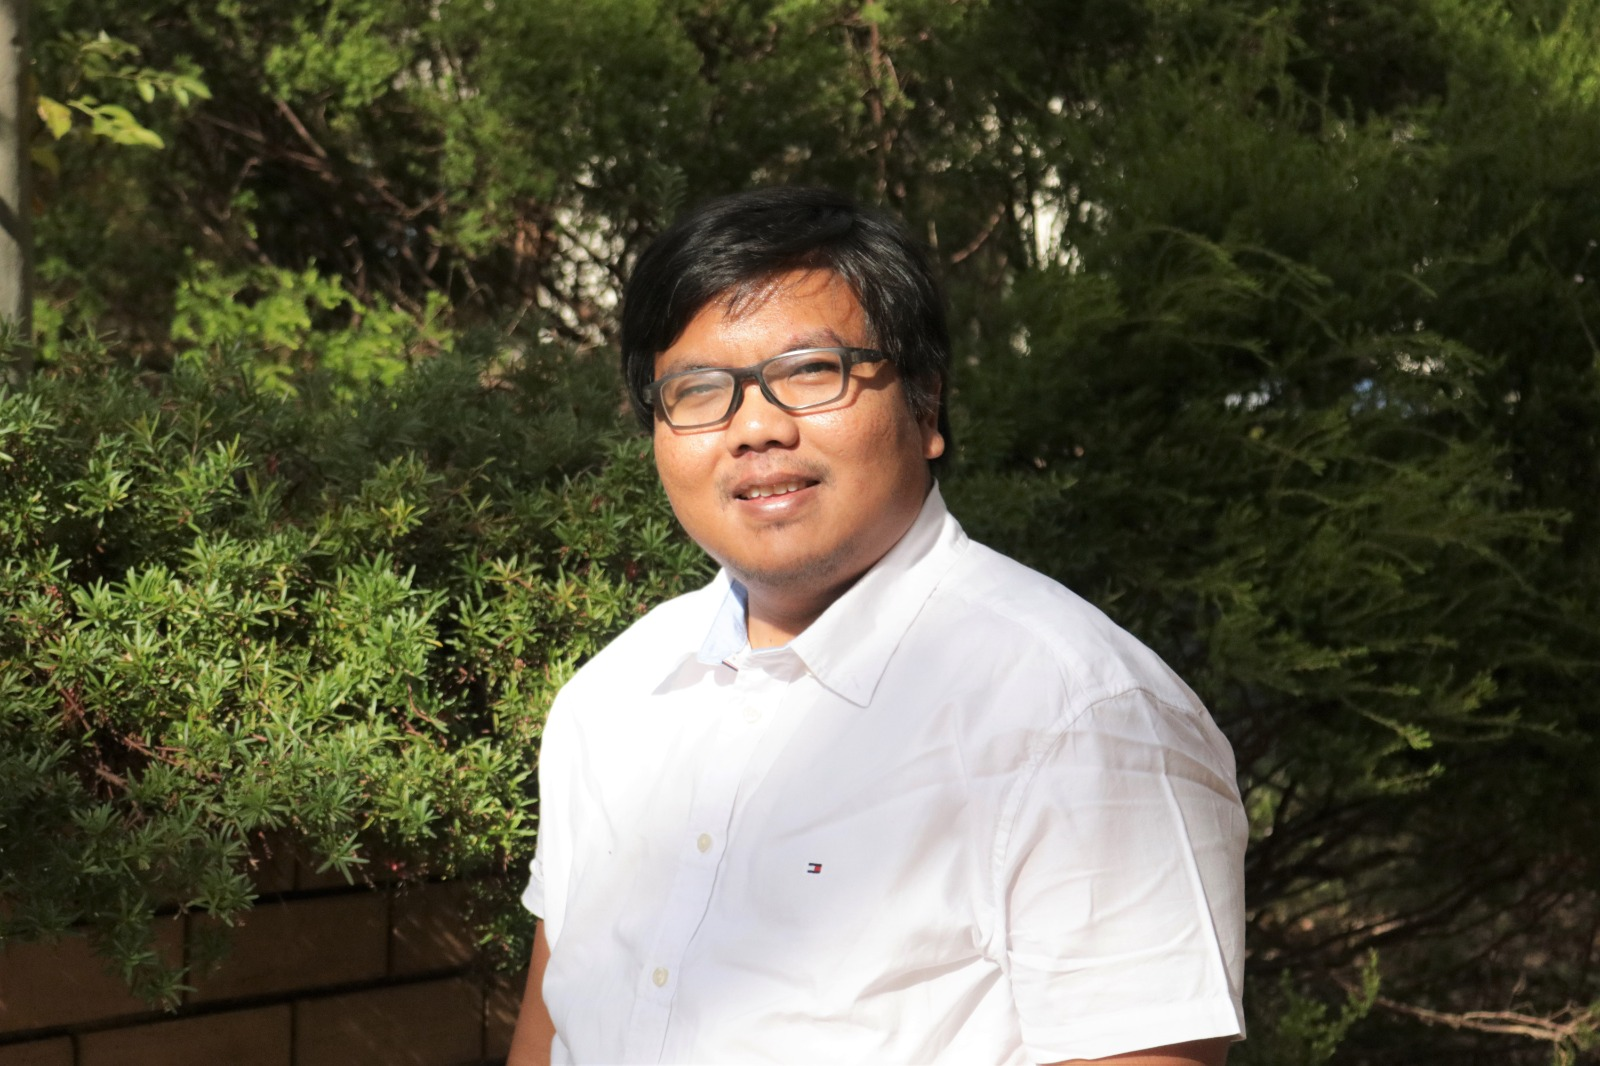
\includegraphics[width=\linewidth]{images/portraits/mahardika_paratama.png} \\[0.5em]
    \begin{center}
        {\textbf{PROF. MAHARDIKA PRATAMA, PH.D}} \\[1em]
        {\normalsize Associate Professor \& Enterprise Fellow in Artificial Intelligence} \\[1em]
        {\normalsize \textbf{Adelaide University Australia}}   
    \end{center}
\end{minipage}%
\hfill
% --- RIGHT COLUMN ---
\begin{minipage}[t]{0.72\textwidth}
    \vspace{0pt}% 
    Professor Mahardhika Pratama is an Associate Professor (Reader) and Enterprise Fellow in Artificial Intelligence at the School of Computer Science and IT, Adelaide University, Australia, and an Adjunct Professor at Institut Teknologi Sepuluh Nopember (ITS), Indonesia. He is a Senior Member of the IEEE and has held academic positions at leading universities in Australia and Singapore, including the Adelaide University, Nanyang Technological University, La Trobe University, and the University of Technology Sydney.

    \vspace{1em}
    
    His research expertise lies in Artificial Intelligence and Machine Learning, with particular emphasis on continual learning, stream learning, few-shot learning, domain adaptation, online learning, and fuzzy neural networks.
    
    \vspace{1em}
    
    Professor Pratama has led and contributed to major research initiatives funded by the Australian Research Council (ARC), SmartSat CRC, Defence Science and Technology Group (DSTG), A*STAR, the National Research Foundation of Singapore, and industry partners. His recent research includes spacecraft autonomy and onboard AI, collaborative autonomy for complex space systems, and dynamic optimization of satellite constellation resources.
    
    \vspace{1em}
    
    He has an extensive publication record in internationally recognized journals and conferences, including IEEE Transactions on Neural Networks and Learning Systems, IEEE Transactions on Fuzzy Systems, Information Sciences, and Knowledge-Based Systems. His research achievements have received international recognition, including the 2024 Outstanding Associate Editor Award from IEEE Transactions on Neural Networks and Learning Systems and the 2019 IEEE Transactions on Fuzzy Systems Publication Award.
    
    \vspace{1em}
    
    Beyond his research, Professor Pratama is an active contributor to the global academic community through editorial leadership, postgraduate supervision, conference organization, and international scholarly engagement. He currently serves as a Senior Editor and Associate Editor for several leading Q1 journals and as a program committee member for major international conferences, including IJCAI, ICLR, ICCV, ECML PKDD, AAAI, and CIKM. He has also delivered numerous keynote and invited presentations internationally on Artificial Intelligence, Machine Learning, data streams, and related areas.
\end{minipage}
% ======================================================================================

\newpage
% --- LEFT COLUMN ---
\large{\textbf{KEYNOTE SPEAKER}}\\
\begin{minipage}[t]{0.25\textwidth}
    \vspace{0pt}%
    
    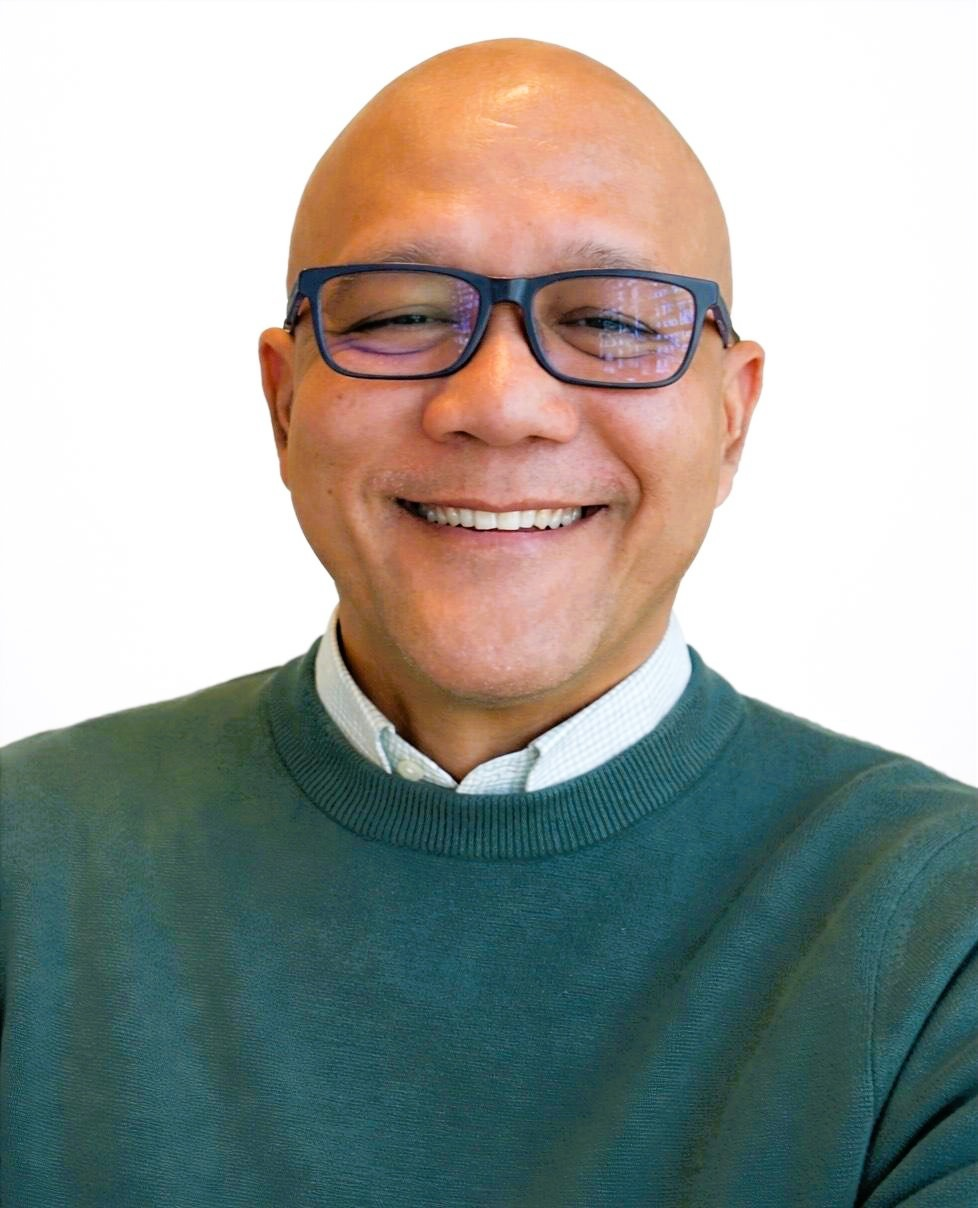
\includegraphics[width=\linewidth]{images/portraits/indra_mahlia.png} \\[0.5em]
    \begin{center}
        {\textbf{PROF. T. M INDRA MAHLIA}} \\[1em]
        {\normalsize Professor of Civil and Environmental Engineering} \\[1em]
        {\normalsize \textbf{University of Technology Sydney Australia}}   
    \end{center}
\end{minipage}%
\hfill
% --- RIGHT COLUMN ---
\begin{minipage}[t]{0.72\textwidth}
    \vspace{0pt}% 
    Professor T M Indra Mahlia is an Australian engineer and a Highly Cited Researcher in the field of Engineering. Currently serving as a Distinguished Professor at the School of Civil and Environmental Engineering, University of Technology Sydney (UTS). He is a key core member of the University’s prestigious Centre for Water and Wastewater Technology (CTWW).
    
    \vspace{1em}
    
    Professor Mahlia’s research interests span a wide range of areas, including Techno-Economic Analysis, Life-Cycle Assessment, Life-Cycle Cost, Cost-Benefit Analysis, Water-Energy Nexus, and Energy \& Fuels.
    
    \vspace{1em}
    
    His dedication to advancing knowledge in these domains has secured over \$6 million in funding for numerous projects supported by government and industrial organisations.
    
    \vspace{1em}
    
    Recognised for his exceptional scholarly achievements, Professor Mahlia has consistently been named a Highly Cited Researcher in Engineering by Clarivate Analytics from 2017 to 2022. Furthermore, The Australian acknowledged his leadership in Sustainable Energy (Engineering \& Computer Science) in a special report published in 2019 and 2025.
    
    \vspace{1em}
    
    Since assuming his role as a Distinguished Professor at UTS in 2018, Professor Mahlia has exhibited a keen interest in mentoring early-career researchers. His guidance and support have been instrumental in fostering the success of his students and fellows.
    
    \vspace{1em}
    
    With his research accomplishments and dedication to nurturing the next generation of scholars, Professor T M Indra Mahlia continues to inspire and shape the field of Engineering, leaving an indelible impact on sustainable energy and environmental engineering.
\end{minipage}
% ======================================================================================

% =============================================================
% Keynote Speaker -- Prof. Andrea Acquaviva
% =============================================================
\newpage
\large{\textbf{KEYNOTE SPEAKER}}\\

\begin{minipage}[t]{0.25\textwidth}
\vspace{0pt}

% Replace with the confirmed portrait:
% \includegraphics[width=\linewidth]{images/portraits/andrea_acquaviva.png}\\[0.5em]

\fbox{
    \parbox[c][4.2cm][c]{\linewidth}{
        \centering
        \small Portrait\\pending
    }
}

\vspace{0.5em}

\begin{center}
{\normalsize \textbf{PROF. ANDREA ACQUAVIVA}}\\[1em]
{\normalsize Keynote Speaker --- Online}\\[1em]
{\normalsize \textbf{Affiliation to be confirmed}}
\end{center}
\end{minipage}%
\hfill
\begin{minipage}[t]{0.72\textwidth}
\vspace{0pt}

Professor Andrea Acquaviva is scheduled to deliver an online keynote address
at IWBIS 2026. His official academic position, institutional affiliation,
biography, and keynote topic will be added upon confirmation.

\vspace{1em}

\textit{This profile is pending confirmation of the speaker's official
biography and approved portrait.}
\end{minipage}

\newpage

% =============================================================
% Keynote Speaker -- Prof. Xiao
% =============================================================
\newpage
\large{\textbf{KEYNOTE SPEAKER}}\\

\begin{minipage}[t]{0.25\textwidth}
\vspace{0pt}

% Replace with the confirmed portrait:
% \includegraphics[width=\linewidth]{images/portraits/prof_xiao.png}\\[0.5em]

\fbox{
    \parbox[c][4.2cm][c]{\linewidth}{
        \centering
        \small Portrait\\pending
    }
}

\vspace{0.5em}

\begin{center}
{\normalsize \textbf{PROF. XIAO}}\\[1em]
{\normalsize Keynote Speaker --- Online}\\[1em]
{\normalsize \textbf{Full name and affiliation to be confirmed}}
\end{center}
\end{minipage}%
\hfill
\begin{minipage}[t]{0.72\textwidth}
\vspace{0pt}

Professor Xiao is scheduled to deliver an online keynote address at IWBIS 2026.
The speaker's full name, professional title, institutional affiliation,
biography, and keynote topic will be announced after confirmation by the
committee.

\vspace{1em}

\textit{This profile is pending confirmation of the speaker's official
identity, biography, and approved portrait.}
\end{minipage}

% =============================================================
% Invited Speaker -- Dr. Henry Edison
% =============================================================
\clearpage
\large{\textbf{INVITED SPEAKER}}\\[0.6em]

\begin{wrapfigure}{l}{0.27\textwidth}
    \vspace{-0.8em}
    \centering

    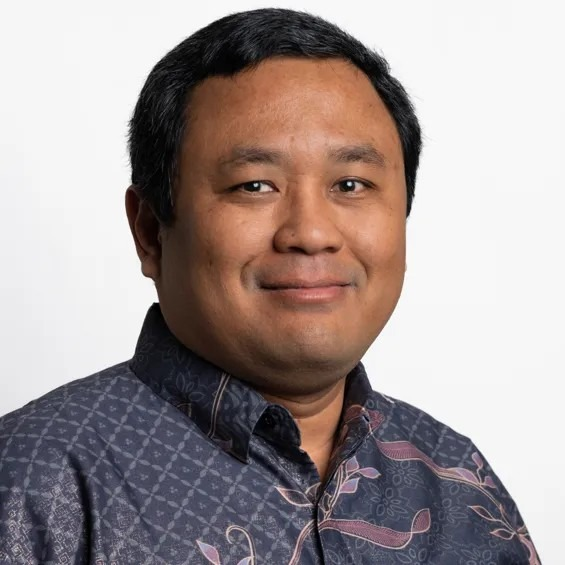
\includegraphics[width=\linewidth]{images/portraits/henri_edion.png}\\[0.6em]

    {\normalsize\bfseries ASSOC.\ PROF.\ HENRY EDISON, PH.D.}\\[0.8em]

    {\small Docent in Software Engineering\\
    and Senior Lecturer}\\[0.8em]

    {\small\bfseries Blekinge Institute of Technology\\
    Sweden}
\end{wrapfigure}

Dr. Henry Edison is a distinguished software engineering scholar and educator
at Blekinge Institute of Technology (BTH), Sweden, where he serves as a Docent
in Software Engineering and Senior Lecturer within the ELLIIT Faculty. With an
international academic career spanning Sweden, Denmark, Ireland, Italy, and
Indonesia, he brings a broad global perspective to software engineering
research, education, and innovation. He holds a PhD in Computer Science from
the Free University of Bozen-Bolzano, Italy, an MSc in Software Engineering
from Blekinge Institute of Technology, Sweden, and a BEng in Informatics from
Institut Teknologi Bandung, Indonesia.

\vspace{1em}

His research focuses on software engineering, digital innovation,
software-intensive businesses, large-scale agile development, and software
startups, with particular attention to how organizations create, develop, and
scale software-intensive products and businesses. His research has been
conducted in close collaboration with international academic and industry
partners, including organizations such as Ericsson, Fidelity Investments,
F-Secure, and Blekinge Business Incubator, connecting rigorous academic inquiry
with real-world challenges in the global software industry.

\vspace{1em}

Dr. Edison is an active contributor to the international software engineering
research community. His academic service includes extensive peer-review
activities, research evaluation, conference and workshop organization, and
program leadership. He has reviewed more than 100 journal, conference, and
workshop submissions since 2016 and has served as an expert evaluator for
research applications for Indonesia's National Research and Innovation Agency.
He has also played a leading role in establishing and organizing international
research forums, including founding the International Workshop on Advances in
Software-Intensive Startups (AiSIS) and serving as Program Chair for the
International Conference on Software Business (ICSOB) 2026.

\vspace{1em}

Beyond research, Dr. Edison has built a substantial international teaching and
academic mentoring portfolio, having taught software engineering and information
systems at universities across Europe and Indonesia since 2005. His teaching and
supervision encompass software engineering, agile and lean development, DevOps,
digital business, strategy and innovation, and sustainability in software
engineering. Through his work with undergraduate, postgraduate, and doctoral
students, he continues to contribute to the development of future researchers,
technology professionals, and academic leaders.

\vspace{1em}

An experienced keynote and invited speaker, Dr. Edison has been invited to
share his expertise at international academic and professional forums on topics
including large-scale agile development, software startups, corporate innovation,
digital business, and academic careers. His combination of international academic
experience, industry engagement, research leadership, and long-standing
contribution to software engineering education positions him as a compelling
voice on the evolution of software-intensive organizations and the future of
software engineering.

\vspace{1em}

With an academic career shaped by collaboration across countries, institutions,
and industry sectors, Dr. Edison brings to the keynote stage not only scholarly
expertise, but also a distinctly international and practice-oriented perspective
on how software engineering continues to transform businesses, organizations,
and society.

\clearpage

% =============================================================
% IWBIS Invited Speaker -- Kamrul Hasan
% =============================================================
\newpage
\large{\textbf{IWBIS INVITED SPEAKER}}\\

\begin{minipage}[t]{0.25\textwidth}
\vspace{0pt}

% Replace with the confirmed portrait:
% \includegraphics[width=\linewidth]{images/portraits/kamrul_hasan.png}\\[0.5em]

\fbox{
    \parbox[c][4.2cm][c]{\linewidth}{
        \centering
        \small Portrait\\pending
    }
}

\vspace{0.5em}

\begin{center}
{\normalsize \textbf{KAMRUL HASAN}}\\[1em]
{\normalsize Invited Speaker}\\[1em]
{\normalsize \textbf{Affiliation to be confirmed}}
\end{center}
\end{minipage}%
\hfill
\begin{minipage}[t]{0.72\textwidth}
\vspace{0pt}

Kamrul Hasan is an invited speaker for the International Workshop on Big Data
and Information Security (IWBIS) 2026. His official professional title,
institutional affiliation, and biography will be announced by the committee.

\vspace{1em}

\textit{This profile is pending confirmation of the speaker's official
biography and approved portrait.}
\end{minipage}

% =============================================================
% IWBIS Invited Speaker -- Grafika Jati
% =============================================================
\newpage
\large{\textbf{IWBIS INVITED SPEAKER}}\\

\begin{minipage}[t]{0.25\textwidth}
\vspace{0pt}

% Replace with the confirmed portrait:
% \includegraphics[width=\linewidth]{images/portraits/grafika_jati.png}\\[0.5em]

\fbox{
    \parbox[c][4.2cm][c]{\linewidth}{
        \centering
        \small Portrait\\pending
    }
}

\vspace{0.5em}

\begin{center}
{\normalsize \textbf{GRAFIKA JATI}}\\[1em]
{\normalsize Invited Speaker --- Online}\\[1em]
{\normalsize \textbf{Affiliation to be confirmed}}
\end{center}
\end{minipage}%
\hfill
\begin{minipage}[t]{0.72\textwidth}
\vspace{0pt}

Grafika Jati is scheduled as an online invited speaker for IWBIS 2026. The
official biography, professional title, institutional affiliation, and session
details will be updated once confirmed by the speaker and the committee.

\vspace{1em}

\textit{This profile is pending confirmation of the speaker's official
biography and approved portrait.}
\end{minipage}

% ====================
% Registration
% ====================
\clearpage
\section*{\textbf{Registration}}
\color{conf}\rule{\linewidth}{1pt}\color{black}
\vspace{0.8em}

\subsection*{\color{conf}Registration Fee of IWBIS 2026}

\small
\renewcommand{\arraystretch}{1.25}
\setlength{\tabcolsep}{5pt}

\textbf{International Participants (USD)}

\vspace{0.3em}

\begin{center}
\begin{tabularx}{\textwidth}{
    >{\raggedright\arraybackslash}p{2.0cm}
    >{\raggedright\arraybackslash}p{1.35cm}
    >{\centering\arraybackslash}X
    >{\centering\arraybackslash}X
    >{\centering\arraybackslash}X
    >{\centering\arraybackslash}X
    >{\centering\arraybackslash}p{1.35cm}
}
\rowcolor{conf}
\multicolumn{2}{c}{\color{white}\textbf{Category}} &
\multicolumn{2}{c}{\color{white}\textbf{Presenter}} &
\multicolumn{2}{c}{\color{white}\textbf{Student Presenter}} &
\color{white}\textbf{Non-presenter} \\

\rowcolor{lightgraybg}
\textbf{Type} &
\textbf{Attendance} &
\textbf{IEEE} &
\textbf{Non-IEEE} &
\textbf{IEEE} &
\textbf{Non-IEEE} &
\\ \hline

Early Bird & Virtual &
250 & 300 & 225 & 250 & 50 \\

Early Bird & On-site &
350 & 400 & 325 & 350 & 150 \\

Regular & Virtual &
300 & 350 & 250 & 300 & 100 \\

Regular & On-site &
400 & 450 & 350 & 400 & 200 \\
\end{tabularx}
\end{center}

\vspace{0.8em}

\textbf{Domestic Participants (IDR)}

\vspace{0.3em}

\begin{center}
\begin{tabularx}{\textwidth}{
    >{\raggedright\arraybackslash}p{2.0cm}
    >{\raggedright\arraybackslash}p{1.35cm}
    >{\centering\arraybackslash}X
    >{\centering\arraybackslash}X
    >{\centering\arraybackslash}X
    >{\centering\arraybackslash}X
    >{\centering\arraybackslash}p{1.35cm}
}
\rowcolor{conf}
\multicolumn{2}{c}{\color{white}\textbf{Category}} &
\multicolumn{2}{c}{\color{white}\textbf{Presenter}} &
\multicolumn{2}{c}{\color{white}\textbf{Student Presenter}} &
\color{white}\textbf{Non-presenter} \\

\rowcolor{lightgraybg}
\textbf{Type} &
\textbf{Attendance} &
\textbf{IEEE} &
\textbf{Non-IEEE} &
\textbf{IEEE} &
\textbf{Non-IEEE} &
\\ \hline

Early Bird & Virtual &
Rp~2,500,000 &
Rp~3,000,000 &
Rp~2,250,000 &
Rp~2,500,000 &
Rp~500,000 \\

Early Bird & On-site &
Rp~3,500,000 &
Rp~4,000,000 &
Rp~3,250,000 &
Rp~3,500,000 &
Rp~1,500,000 \\

Regular & Virtual &
Rp~2,750,000 &
Rp~3,500,000 &
Rp~2,500,000 &
Rp~3,000,000 &
Rp~750,000 \\

Regular & On-site &
Rp~3,750,000 &
Rp~4,500,000 &
Rp~3,500,000 &
Rp~4,000,000 &
Rp~1,750,000 \\
\end{tabularx}
\end{center}

\normalsize
\vspace{0.7em}

\begin{minipage}{\linewidth}
\small
\textit{IEEE member and non-IEEE member fees appear in that order. Registration fees are per paper. Conference registration includes electronic proceedings, an e-certificate, and access to the IWBIS and ICACSIS 2026 parallel sessions.}
\end{minipage}

\vspace{1.2em}

\clearpage
\subsection*{\color{conf}Payment}

\begin{table}[h]
\centering
\renewcommand{\arraystretch}{1.4}
\begin{tabular}{|l|p{0.75\textwidth}|}
\hline
\multirow{2}{*}{
\includegraphics[width=2cm]{images/bni.png}} &
Bank Name : BNI \newline
Account Name (payee): UNIVERSITAS-INDONESIA \newline
Branch name: UI Depok \newline
Account Number : 127 3000 444 \newline
Swift Code (BIC) : \newline
BNI NIDJA 127 3000 444 for 8 characters \newline
or \newline
BNI NIDJA XXX 127 3000 444 for 11 characters \\ \cline{2-2}
&
Branch name address (with postcode, town, country): Gedung Perpustakaan Pusat Universitas Indonesia, Kampus UI Depok, Depok, Jawa Barat, Indonesia, 16424 \newline
\newline
Address of payee (with postcode, town, country): Fakultas Ilmu Komputer, Kampus UI Depok, Depok, Jawa Barat, Indonesia, 16424 \newline
\newline
Phone number or payee: +62 21 7863419 \\ \hline
\multicolumn{2}{|p{0.9\textwidth}|}{%
There will be additional fees (\$50/page or Rp 883.450/page) if your paper is more than 6 pages, and please be sure that your paper is not more than 10 pages. \newline
\newline
Transfer fees transactions are charged to the author. \newline
\newline
Make sure one of the author(s) of the paper registers to the conference by September 30, 2026, at the latest (September 15, 2026 at the latest for early bird). Please fill in the following form: https://bit.ly/icacsis2026\_regist (Form submission needs to log in from Google account.) \newline
\newline
We do not provide printed proceeding onsite, please contact us if you need one. There is an additional charge to print and ship it to your address
} \\ \hline
\end{tabular}
\end{table}

\vspace{0.8em}

\subsection*{\color{conf}Registration Notes}

\begin{itemize}
    \setlength{\itemsep}{0.4em}
    \item At least one author of each accepted paper must register by \textbf{30 September 2026}.
    \item Authors and non-presenting participants may register at:
    \url{https://bit.ly/iwbis2026-regist}
    \item The registration form requires a Google account.
    \item Virtual registration is available. Details of the Zoom link or meeting ID will be distributed closer to the event.
\end{itemize}

\normalsize


% ====================
% Conference Platform
% ====================
\clearpage
\section*{\textbf{Conference Platform}}
\color{conf}\rule{\linewidth}{1pt}\color{black}
\vspace{0.8em}

\begin{minipage}{\linewidth}
\textbf{\color{conf}ON-SITE PARTICIPATION}

\vspace{0.4em}

The workshop will take place at the \textbf{Faculty of Computer Science, Universitas Indonesia}. The committee will announce the session rooms together with the final program.

\vspace{0.6em}

\renewcommand{\arraystretch}{1.25}
\setlength{\tabcolsep}{10pt}

\begin{center}
\begin{tabularx}{0.95\textwidth}{
    >{\raggedright\arraybackslash}p{4.3cm}
    >{\raggedright\arraybackslash}X
}
\rowcolor{lightgraybg}
\textbf{Activity} & \textbf{Venue} \\

Plenary and keynote sessions &
Auditorium Indro Suwandi \\

Parallel sessions &
Classrooms, Level 2, Zone 3; and Sidang rooms \\
\end{tabularx}
\end{center}

\vspace{0.4em}

Detailed room assignments for each session will be communicated with the final program.

\end{minipage}

\vspace{1.2em}

\begin{minipage}{\linewidth}
\textbf{\color{conf}VIRTUAL PARTICIPATION}

\vspace{0.4em}

Virtual registration is available. The conference will use the \textbf{Zoom} platform (\url{https://zoom.us}).

\vspace{0.6em}

\begin{itemize}
    \setlength{\itemsep}{0.35em}
    \item All plenary and keynote sessions will be livestreamed through Zoom.
    \item Several invited and keynote speakers will also participate online, including the IWBIS Invited Speaker session with Grafika.
    \item The Zoom meeting link and/or meeting ID will be shared closer to the event.
\end{itemize}

\end{minipage}

% ====================
% Technical Program
% ====================
\clearpage
\section*{\textbf{Technical Program}}
\color{conf}\rule{\linewidth}{1pt}\color{black}
\vspace{0.6em}

The detailed technical program below is scheduled for \textbf{Sunday, 18 October 2026},
from \textbf{10:00 to 11:45 GMT+7}. Each presentation is allocated
\textbf{20 minutes}, including 15 minutes for the presentation and 5 minutes
for questions, answers, and transition.

\vspace{0.8em}

% ------------------------------------------------------------
% Parallel Session 1
% ------------------------------------------------------------
\subsection*{\color{conf}Parallel Session 1: Cybersecurity \& Cryptography}

\begin{tabularx}{\textwidth}{
    >{\raggedright\arraybackslash}p{3.4cm}
    >{\raggedright\arraybackslash}X
}
\rowcolor{lightgraybg}
\textbf{Time} & 10:00--11:45 GMT+7 \\

\rowcolor{lightgraybg}
\textbf{Session Chair} & TBD \\

\rowcolor{lightgraybg}
\textbf{Location} & TBD --- Classroom, Level 2, Zone 3 / Sidang Room \\
\end{tabularx}

\vspace{0.5em}

\small
\renewcommand{\arraystretch}{1.25}
\setlength{\tabcolsep}{5pt}

\begin{longtable}{
    |>{\centering\arraybackslash}p{0.7cm}
    |>{\raggedright\arraybackslash}p{8.2cm}
    |>{\raggedright\arraybackslash}p{5.0cm}|
}
\hline
\rowcolor{conf}
\color{white}\textbf{No.} &
\color{white}\textbf{Paper Title} &
\color{white}\textbf{Authors} \\
\hline
\endfirsthead

\hline
\rowcolor{conf}
\color{white}\textbf{No.} &
\color{white}\textbf{Paper Title} &
\color{white}\textbf{Authors} \\
\hline
\endhead

1 &
\textit{Latviz: A Process Visualization for ML-KEM, ML-DSA, and Lattice-Based Cryptanalysis Using LLL and BKZ} &
Jeslyn Theodora; Muhammad Imam Chaidar Mujaddid Al-Ghiffari; Amril Syalim \newline
\textcolor{gray}{Universitas Indonesia} \\
\hline

2 &
\textit{Channel-Aware Backdoor Attacks Against Federated Infostealer Malware Classification Using Dynamic API-Call and Network Representations} &
Mochamad Asryl Aziz \newline
\textcolor{gray}{BPS Bantaeng}; Moh. Jabir Mubarok \newline
\textcolor{gray}{Institut Teknologi Sepuluh Nopember}; Eka Fitria \newline
\textcolor{gray}{Universitas Syiah Kuala} \\
\hline

3 &
\textit{Real-Time Security Monitoring Hub with Telegram Bot API Integration for Instant Threat Alerting in a Laravel-Based Corporate Web Application} &
Yakhof Kalladzi Mustohar Bahaudin \newline
\textcolor{gray}{President University} \\
\hline

4 &
\textit{A Human-in-the-Loop Approach to Capturing the Challenges Posed by Hidden Online Gambling Promotion Sites in Indonesia} &
Abdul Azzam Ajhari \newline
\textcolor{gray}{Universitas Indonesia / UNSIA}; Rizal Fathoni Aji; Aprinaldi Jasa Mantau; Wisnu Jatmiko \newline
\textcolor{gray}{Universitas Indonesia} \\
\hline

5 &
\textit{Analysis and Implementation of the Lattice-Based Quantum-Resistant Digital Signature Algorithm CRYSTALS-Dilithium} &
Dhafin Fadhlan Kamal \newline
\textcolor{gray}{Universitas Indonesia} \\
\hline
\end{longtable}
\normalsize

% ------------------------------------------------------------
% Parallel Session 2
% ------------------------------------------------------------
\clearpage
\subsection*{\color{conf}Parallel Session 2: NLP \& Analytics}

\begin{tabularx}{\textwidth}{
    >{\raggedright\arraybackslash}p{3.4cm}
    >{\raggedright\arraybackslash}X
}
\rowcolor{lightgraybg}
\textbf{Time} & 10:00--11:45 GMT+7 \\

\rowcolor{lightgraybg}
\textbf{Session Chair} & TBD \\

\rowcolor{lightgraybg}
\textbf{Location} & TBD --- Classroom, Level 2, Zone 3 / Sidang Room \\
\end{tabularx}

\vspace{0.5em}

\small
\renewcommand{\arraystretch}{1.25}
\setlength{\tabcolsep}{5pt}

\begin{longtable}{
    |>{\centering\arraybackslash}p{0.7cm}
    |>{\raggedright\arraybackslash}p{8.2cm}
    |>{\raggedright\arraybackslash}p{5.0cm}|
}
\hline
\rowcolor{conf}
\color{white}\textbf{No.} &
\color{white}\textbf{Paper Title} &
\color{white}\textbf{Authors} \\
\hline
\endfirsthead

\hline
\rowcolor{conf}
\color{white}\textbf{No.} &
\color{white}\textbf{Paper Title} &
\color{white}\textbf{Authors} \\
\hline
\endhead

1 &
\textit{Geospatial Sentiment Analysis and Interactive Mapping of Hospital Services Using Support Vector Machine} &
Boutefhika Nuha Ziyadatul Khair; Andika Neviantoro; Sudianto \newline
\textcolor{gray}{Telkom University} \\
\hline

2 &
\textit{Geographic Sentiment Patterns and Venue-Level Variability in Cafe Reviews Using Machine Learning} &
Jordan Angkawijaya; Naswa Malika Putri; Sudianto \newline
\textcolor{gray}{Telkom University} \\
\hline

3 &
\textit{Do AI Models Reflect Indonesian Values? A Probe-Based Audit of Collectivism-Individualism Bias in Foundation Models} &
Abdul Aziz; Muhammad Hatta Eka Putra; Aris Budi Santoso; Indra Budi \newline
\textcolor{gray}{Universitas Indonesia} \\
\hline

4 &
\textit{Interpretable Detection of Psychological Distress Tendency on Reddit Using Hybrid Linguistic and DSM-5 Features with MentalBERT} &
Supriadi; Ika Alfina; Evi Yulianti; Grafika Jati; Wisnu Jatmiko \newline
\textcolor{gray}{Universitas Indonesia; University of Bologna, FEV, Italy} \\
\hline

5 &
\textit{A Comparative Study of Pretrained Language Models Under Varying Training Data Sizes for Sentiment Analysis in Indonesian Local Languages} &
Willy Wilsen; Ika Alfina; Evi Yulianti; Nur Hamid; Wisnu Jatmiko \newline
\textcolor{gray}{Universitas Indonesia; King Fahd University of Petroleum and Minerals} \\
\hline
\end{longtable}
\normalsize

% ------------------------------------------------------------
% Parallel Session 3
% ------------------------------------------------------------
\clearpage
\subsection*{\color{conf}Parallel Session 3: Computer Vision, Data Structure \& Governance}

\begin{tabularx}{\textwidth}{
    >{\raggedright\arraybackslash}p{3.4cm}
    >{\raggedright\arraybackslash}X
}
\rowcolor{lightgraybg}
\textbf{Time} & 10:00--11:45 GMT+7 \\

\rowcolor{lightgraybg}
\textbf{Session Chair} & Erdefi Rakun --- not yet confirmed \\

\rowcolor{lightgraybg}
\textbf{Location} & TBD --- Classroom, Level 2, Zone 3 / Sidang Room \\
\end{tabularx}

\vspace{0.5em}

\small
\renewcommand{\arraystretch}{1.25}
\setlength{\tabcolsep}{5pt}

\begin{longtable}{
    |>{\centering\arraybackslash}p{0.7cm}
    |>{\raggedright\arraybackslash}p{8.2cm}
    |>{\raggedright\arraybackslash}p{5.0cm}|
}
\hline
\rowcolor{conf}
\color{white}\textbf{No.} &
\color{white}\textbf{Paper Title} &
\color{white}\textbf{Authors} \\
\hline
\endfirsthead

\hline
\rowcolor{conf}
\color{white}\textbf{No.} &
\color{white}\textbf{Paper Title} &
\color{white}\textbf{Authors} \\
\hline
\endhead

1 &
\textit{Blockchain Adoption Challenges in Finance: A Comparative Study of Banking and Insurance Sectors} &
Isyrofi Susianto \newline
\textcolor{gray}{Universitas Indonesia}; Geri Yesa Ermawan \newline
\textcolor{gray}{Politeknik Statistika STIS}; Setiadi Yazid \newline
\textcolor{gray}{Universitas Indonesia} \\
\hline

2 &
\textit{Table Detection in Document Images with Borderless and Partially Ruled Layouts: A Step Toward Table Understanding} &
Alvin Sarraga; Alon Adamson \newline
\textcolor{gray}{University of De La Salle} \\
\hline

3 &
\textit{Attention-Enhanced Dense U-Net for Road and Building Segmentation in High-Resolution Aerial Imagery} &
Gilang Mantara Putra \newline
\textcolor{gray}{Universitas Indonesia}; Muhammad Anwar Masum \newline
\textcolor{gray}{Adelaide University}; Laksmita Rahadianti; Aniati M. Arymurthy; Wisnu Jatmiko \newline
\textcolor{gray}{Universitas Indonesia} \\
\hline

4 &
\textit{Agentic AI on National Digital Identity Big Data: Extending the FrontCRM Framework for Citizen Relationship Management} &
Wira Perdana; Muhammad Nuh Al Azhar; Eko K. Budiardjo; Wisnu Jatmiko \newline
\textcolor{gray}{Universitas Indonesia} \\
\hline

5 &
\textit{Model-Based Parameter Optimization for Bloom Filter and Cuckoo Filter Under Dynamic Workloads} &
Nyoman Purnama \newline
\textcolor{gray}{Universitas Primakara}; Sudarma Made; Nyoman Putra Sastra; Dewa Wiharta \newline
\textcolor{gray}{Udayana University} \\
\hline
\end{longtable}
\normalsize

% ====================
% Presenter Guidelines
% ====================
\clearpage
\section*{\textbf{Guidelines for Presenters}}
\color{conf}\rule{\linewidth}{1pt}\color{black}
\vspace{0.8em}

\subsection*{\color{conf}1. Presentation Time and Format}

\begin{itemize}[leftmargin=*, noitemsep]
    \item \textbf{Presentation duration.} Each paper is allocated a total of
    \textbf{20 minutes}, comprising 15 minutes for the presentation and
    5 minutes for questions, answers, and transition.

    \item \textbf{Language.} All presentations and presentation slides must be
    delivered in English.

    \item \textbf{Slide format.} Please prepare your presentation slides in
    \textbf{16:9 widescreen} aspect ratio.
\end{itemize}

\vspace{0.8em}

\subsection*{\color{conf}2. Onsite Presenters}

\begin{itemize}[leftmargin=*, noitemsep]
    \item \textbf{Reporting time.} Arrive at your assigned session room at least
    \textbf{10--15 minutes} before the scheduled session starts.

    \item \textbf{Session check-in.} Introduce yourself to the Session Chair and
    test your presentation before the session begins.

    \item \textbf{Available equipment.} A laptop, projector, and audio system
    will be provided in each session room.

    \item \textbf{File submission.} Copy your final presentation file in PDF or
    PowerPoint (\texttt{.pptx}) format to the session-room laptop using a USB
    drive before the session begins or during the preceding break.
\end{itemize}

\vspace{0.8em}

\subsection*{\color{conf}3. Virtual Presenters}

\begin{itemize}[leftmargin=*, noitemsep]
    \item \textbf{Platform.} Virtual presentations will be conducted through Zoom.

    \item \textbf{Pre-session setup.} Join the assigned Zoom room at least
    \textbf{10 minutes} before your session to test your microphone, camera,
    and screen-sharing function.

    \item \textbf{Display name.} Use the following Zoom display-name format:
    \texttt{Paper ID - Presenter Name}. For example:
    \texttt{101 - Jane Doe}.

    \item \textbf{Technical readiness.} Use a stable internet connection, a quiet
    presentation environment, and a properly functioning headset or microphone.
\end{itemize}

% ====================
% Session Chair Guidelines
% ====================
\clearpage
\section*{\textbf{Guidelines for Session Chairs}}
\color{conf}\rule{\linewidth}{1pt}\color{black}
\vspace{0.8em}

\subsection*{\color{conf}1. Before the Session}

\begin{itemize}[leftmargin=*, noitemsep]
    \item \textbf{Check-in.} Arrive at the assigned session room for onsite
    participation, or join the Zoom room for virtual participation, at least
    \textbf{15 minutes} before the session begins.

    \item \textbf{Presenter attendance.} Verify that all presenters assigned to
    the session are present, including both onsite and virtual presenters.

    \item \textbf{Presentation materials.} Ensure that onsite presentation files
    are available on the session-room computer.

    \item \textbf{Virtual readiness.} Confirm that virtual presenters have been
    granted the necessary co-host and/or screen-sharing permissions.
\end{itemize}

\vspace{0.8em}

\subsection*{\color{conf}2. During the Session}

\begin{itemize}[leftmargin=*, noitemsep]
    \item \textbf{Introduction.} Open the session promptly at the scheduled time,
    announce the session topic, and introduce each presenter before their talk.

    \item \textbf{Time management.} Maintain the allocation of \textbf{20 minutes}
    per paper: 15 minutes for the presentation and 5 minutes for questions,
    answers, and transition.

    \item \textbf{Time warnings.} Give each presenter clear time reminders, for
    example when three minutes and one minute remain.

    \item \textbf{Schedule discipline.} Do not allow presentations to exceed the
    allocated time, in order to preserve fairness and maintain the published
    schedule.

    \item \textbf{Question-and-answer moderation.} Facilitate questions from both
    onsite participants and virtual attendees, including questions submitted
    through Zoom chat or raised-hand features.

    \item \textbf{Backup question.} If no questions are raised by the audience,
    prepare at least one relevant question for the presenter.
\end{itemize}

\vspace{0.8em}

\subsection*{\color{conf}3. No-Shows and Cancellations}

\begin{itemize}[leftmargin=*, noitemsep]
    \item \textbf{Fixed schedule.} Do not advance the start times of subsequent
    presentations when an author is absent or a paper is cancelled.

    \item \textbf{Use of vacant slots.} Maintain the official schedule so that
    participants joining for a specific paper can attend at the announced time.
    A vacant slot may be used for a short discussion or recess.
\end{itemize}

\vspace{0.8em}

\subsection*{\color{conf}4. After the Session}

\begin{itemize}[leftmargin=*, noitemsep]
    \item \textbf{Attendance and evaluation.} Record presenter attendance and
    complete the Session Evaluation and Best Presenter Recommendation form
    provided by the committee.

    \item \textbf{Closing.} Thank the presenters and audience, then formally
    conclude the session.
\end{itemize}

% ======== End Cover
\newpage
\thispagestyle{empty}
\AddToShipoutPictureBG*{%
  \includegraphics[width=\paperwidth,height=\paperheight]{assets/cover_page_b.pdf}%
}


\begin{tikzpicture}[remember picture, overlay]
   \node[anchor=north, text width=150mm, align=center]
    at ([yshift=-70mm]current page.north)
    {\Huge\bfseries IWBIS \\[0.5cm]  2026};

  \node[anchor=north west, text width=60mm, align=left]
    at ([xshift=2cm,yshift=-21.5cm]current page.north west)
    {\large Contact Us:\\
    Faculty of Computer Science\\
    Universitas Indonesia\\
    Kampus UI Depok, Indonesia 16424\\
    Telp: +62 21 786 3419\\
    Fax: +62 21 786 3415\\
    Email: iwbis@cs.ui.ac.id\\
    Website: iwbis.cs.ui.ac.id
    };
\end{tikzpicture}

\end{document}